% !TeX program = lualatex
%******************************************************** -*-LaTeX-*- ******************************
%                                                                                                  *
% v1.1.2.6.8 Acht.tex                                                                              *
%                                                                                                  *
% Copyright (C) 2023 Kategory GmbH \& Co. KG (joerg.kunze@kategory.de)                             *
%                                                                                                  *
% v1.1.2.6.8 is part of kategoryMathematik.                                                        *
%                                                                                                  *
% kategoryMathematik is free software: you can redistribute it and/or modify                       *
% it under the terms of the GNU General Public License as published by                             *
% the Free Software Foundation, either version 3 of the License, or                                *
% (at your option) any later version.                                                              *
%                                                                                                  *
% kategoryMathematik is distributed in the hope that it will be useful,                            *
% but WITHOUT ANY WARRANTY; without even the implied warranty of                                   *
% MERCHANTABILITY or FITNESS FOR A PARTICULAR PURPOSE.  See the                                    *
% GNU General Public License for more details.                                                     *
%                                                                                                  *
% You should have received a copy of the GNU General Public License                                *
% along with this program.  If not, see <http://www.gnu.org/licenses/>.                            *
%                                                                                                  *
%***************************************************************************************************

% !!!!!!!!!!!!!!!!!!!!!!!!!!!!!!!!!!!!!!!!!!!!!!!!!!!!!!!!!!!!!!!!!!!!!!!!!!!!!!!!!!!!!!!!!!!!!!!
% Wegen der hebräischen Schrift geht diese Datei nunr mit LuaLaTeX.
% deswegen die erste Zeile, damit TeXstudio den LuaLaTeX-Compiler nimmt
% Zusätzlich müssen wir den SBL Hebrew FOnt isntallieren.
% Den finden wir unter https://www.sbl-site.org/educational/biblicalfonts_sblhebrew.aspx
% Nach dem Download muss die Datei SBL_Hbrw.ttf in das Verzeichniss c:\Windows\Fonts kopiert werden
% Das ist aber auch im auf der selben Web-Seite zu findenen User Manual beschrieben.
% Wie es auf Linux oder Mac geht, können wir auch dort beschrieben finden. 
% Achte auch auf das \usepackage[utf8]{luainputenc}

\documentclass[a4paper]{amsart}
% \documentclass[a4paper]{book}

%-----------------------------------------------------------------------------------------------------*
% package:                                                                                            *
%-----------------------------------------------------------------------------------------------------*
\usepackage{amssymb}
\usepackage{amsfonts}
\usepackage{amsmath}
\usepackage{amsthm}

\usepackage{mathabx}

\usepackage{a4wide} % a little bit smaller margins

\usepackage{graphicx}
\usepackage{hyperref}
\usepackage{algorithmic}
\usepackage{listings}
\usepackage{color}
\usepackage{colortbl}
\usepackage{sidecap}
\usepackage{comment}
\usepackage{tcolorbox}
\usepackage{collect}

\usepackage{upgreek}

% \usepackage{diagrams}
\usepackage{luatextra}

\usepackage{polyglossia}
\usepackage[autostyle,german=guillemets]{csquotes}

\setmainlanguage[spelling=new]{german}
\setotherlanguage[variant=polytonic]{greek}

\newfontfamily\hebrewfont[Script=Hebrew,Scale=MatchUppercase,Ligatures=TeX]{SBL Hebrew}
\newcommand{\texthebrew}[1]{\bgroup\textdir TRT\hebrewfont #1\egroup}
\newenvironment{hebrew}{\textdir TRT\pardir TRT\hebrewfont}{}

\usepackage[none]{hyphenat}
\emergencystretch=4em

\usepackage[utf8]{luainputenc} % to be able to use äöü as characters in text
\usepackage[T1]{fontenc} % to be able to use äöü in lables
\usepackage{lmodern}     % to avoid pixelation introduced by fontenc

\usepackage{hyperref}

\usepackage{tikz}
\usepackage{tikz-cd}
\usetikzlibrary{shapes.geometric}

\usetikzlibrary{babel}

%-----------------------------------------------------------------------------------------------------*
% theorem:                                                                                            *
%-----------------------------------------------------------------------------------------------------*
\theoremstyle{definition}
\newtheorem{theorem}{Theorem}[subsection]

\newcommand{\myTheorem}[1]{%
  \newtheorem{jk#1}[theorem]{#1}
  \newenvironment{#1}[1]{%
    \expandafter\begin{jk#1} \expandafter\label{#1:##1}\textbf{(##1):}
  }{%
    \expandafter\end{jk#1}
  }
}

\myTheorem{Definition}
\myTheorem{Proposition}
\myTheorem{Theorem}
\myTheorem{Example}
\myTheorem{Remark}

\definecollection{jkjkFrage}
\newtheorem{jkFrage}[theorem]{Frage}
\newenvironment{Frage}[1]{%
  \expandafter\begin{jkFrage} \expandafter\label{Frage:#1}\textbf{(#1):}
  \begin{collect}{jkjkFrage}{}{}
    \item \ref{Frage:#1} #1
  \end{collect}
}{%
  \expandafter\end{jkFrage}
}

\newcommand{\myRef}[2]{[#1 \ref{#1:#2}, ``#2'']}

\renewcommand{\proofname}{Beweis}

%-----------------------------------------------------------------------------------------------------*
% operator:                                                                                           *
%-----------------------------------------------------------------------------------------------------*
\DeclareMathOperator{\End}{End}
\DeclareMathOperator{\Ker}{Ker}
\DeclareMathOperator{\Mat}{Mat}
\DeclareMathOperator{\rank}{rank}
\DeclareMathOperator{\ggT}{ggT}
\DeclareMathOperator{\len}{len}
\DeclareMathOperator{\ord}{ord}
\DeclareMathOperator{\kgV}{kgV}
\DeclareMathOperator{\id}{id}
\DeclareMathOperator{\red}{red}
\DeclareMathOperator{\supp}{supp}
\DeclareMathOperator{\Bild}{Bild}
\DeclareMathOperator{\Rang}{Rang}
\DeclareMathOperator{\Det}{Det}
\DeclareMathOperator{\Hom}{Hom}

\DeclareMathOperator{\sub}{sub}
\DeclareMathOperator{\blk}{blk}
\DeclareMathOperator{\minimal}{minimal}
\DeclareMathOperator{\maximal}{maximal}

\definecolor{mygreen}{rgb}{0,0.6,0}
\definecolor{mygray}{rgb}{0.5,0.5,0.5}
\definecolor{mymauve}{rgb}{0.58,0,0.82}

\lstset{ %
  backgroundcolor=\color{white},   % choose the background color
  basicstyle=\ttfamily\footnotesize,        % size of fonts used for the code
  breaklines=true,                 % automatic line breaking only at whitespace
  captionpos=b,                    % sets the caption-position to bottom
  commentstyle=\color{mygreen},    % comment style
  escapeinside={\%*}{*)},          % if you want to add LaTeX within your code
  keywordstyle=\color{blue},       % keyword style
  stringstyle=\color{mymauve},     % string literal style
  frame=single
}

\setcounter{MaxMatrixCols}{20}

%******************************************************************************************************
%                                                                                                     *
% definition:                                                                                         *
%                                                                                                     *
%******************************************************************************************************
\newcommand{\R}{\ensuremath{\mathbb{ R }}}
\newcommand{\Q}{\ensuremath{\mathbb{ Q }}}
\newcommand{\Z}{\ensuremath{\mathbb{ Z }}}
\newcommand{\N}{\ensuremath{\mathbb{ N }}}
\newcommand{\C}{\ensuremath{\mathbb{ C }}}
\newcommand{\A}{\ensuremath{\mathbb{ A }}}
\newcommand{\F}{\ensuremath{\mathbb{ F }}}
\newcommand{\K}{\ensuremath{\mathbb{ K }}}
\newcommand{\Pb}{\ensuremath{\mathbb{ P }}}

\newcommand{\M}{\ensuremath{\mathcal{ M }}}
\newcommand{\V}{\ensuremath{\mathcal{ V }}}

\newcommand{\AAA}{\ensuremath{\mathcal{ A }}}
\newcommand{\BB}{\ensuremath{\mathcal{ B }}}
\newcommand{\CC}{\ensuremath{\mathcal{ C }}}
\newcommand{\EE}{\ensuremath{\mathcal{ E }}}
\newcommand{\KK}{\ensuremath{\mathcal{ K }}}
\newcommand{\MM}{\ensuremath{\mathcal{ M }}}
\newcommand{\PP}{\ensuremath{\mathcal{ P }}}
\newcommand{\ZZ}{\ensuremath{\mathcal{ Z }}}

\newcommand{\imporant}[1]{ \textcolor{red}{\textbf{#1}} }

\newcommand{\bb}[1]{\mathbf{#1}}
\newcommand{\balpha}{\boldsymbol{\upalpha}}
\newcommand{\bbeta}{\boldsymbol{\upbeta}}
\newcommand{\bgamma}{\boldsymbol{\upgamma}}
\newcommand{\bdelta}{\boldsymbol{\delta}}
\newcommand{\bmu}{\boldsymbol{\upmu}}

\newcommand{\z}[1]{\Z_{#1}}
\newcommand{\e}[1]{\z{#1}^*}
\newcommand{\q}[1]{(\e{#1})^2}

\excludecomment{book}
\excludecomment{example}
\excludecomment{backup}

\begin{document}

%******************************************************************************************************
%                                                                                                     *
\begin{titlepage}
%                                                                                                     *
%******************************************************************************************************
% \vspace*{\fill}
\centering
{\huge
(Grund) Zahlen\\[1cm]
\textbf{v1.1.2.6.8 Acht}
}\\[1cm]

\textbf{Kategory GmbH \& Co. KG}\\
Präsentiert von Jörg Kunze

\end{titlepage}

%\clearpage
%\setcounter{page}{2}
%
%\tableofcontents

\newpage

%******************************************************************************************************
%                                                                                                     *
\section*{Beschreibung}
%                                                                                                     *
%******************************************************************************************************

%******************************************************************************************************
\subsection*{Inhalt}
%******************************************************************************************************
Die ||||| ||| (8, Acht) ist der Nachfolger von ||||| || (7, Sieben). Die Acht ist die erste und damit kleinste Zahl, die drei Faktoren hat. Deswegen lässt sie sich in mehrere gleich große Rechtecke aufteilen und sie ist die kleinste Zahl mit dieser Eigenschaft. Aus dem selben Grund ist das Achteck sehr symmetrisch.

Das Stoppschild ist achteckig. Oktopusse (Kraken) haben acht Beine. Spinnen auch.

%******************************************************************************************************
\subsection*{Präsentiert}
%******************************************************************************************************
Von Jörg Kunze

%******************************************************************************************************
\subsection*{Voraussetzungen}
%******************************************************************************************************
Schulmathematik, Zählen, ein wenig rechnen mit Strichen und Punkten, Zählen, Addieren, Pack-Schreibweise von Zahlen.

%******************************************************************************************************
\subsection*{Text}
%******************************************************************************************************
Der Begleittext als PDF und als LaTeX findet sich unter
\url{}.

%******************************************************************************************************
\subsection*{Meine Videos}
%******************************************************************************************************
Siehe auch in den folgenden Videos:\\
v1.1.2.5.6.1 (Grund) Zahlen - Darstellung\\
\url{https://youtu.be/t8cyZevFWFs}\\
\\
v1.1.2.5.6 (Grund) Zahlen - Pack Schreibweise\\
\url{https://youtu.be/OGXoLiBL2MQ}\\
\\
v1.1.2.4 (Grund) Zählen\\
\url{ttps://youtu.be/I6iIG2ZtPCU}\\

%******************************************************************************************************
\subsection*{Quellen}
%******************************************************************************************************
Siehe auch in den folgenden Seiten:\\
\url{https://de.wikipedia.org/wiki/Acht}\\
\url{https://de.wikipedia.org/wiki/Echte_Kraken}\\
\url{https://de.wikipedia.org/wiki/Stoppschild}\\
\url{https://de.wikipedia.org/wiki/Achteck}

%******************************************************************************************************
\subsection*{Buch}
%******************************************************************************************************
Grundlage ist folgendes Buch:\\
"`Basiswissen Grundschule – Mathematik"'\\
Ute Müller-Wolfangel, Beate Schreiber\\
2014\\
Bibliographisches Institut\\
978-3-411-72063-7 (ISBN)
\\
\url{https://www.lehmanns.de/shop/schulbuch-lexikon-woerterbuch/28535581-9783411720637-basiswissen-grundschule-mathematik}

%******************************************************************************************************
%                                                                                                     *
\section{Acht}
%                                                                                                     *
%******************************************************************************************************
\def\kategoryVspace{5pt}

%******************************************************************************************************
\subsection{Striche}
%******************************************************************************************************
\begin{tikzpicture}
\draw (0.0, 0) -- (0.0, 0.4);
\draw (0.1, 0) -- (0.1, 0.4);
\draw (0.2, 0) -- (0.2, 0.4);
\draw (0.3, 0) -- (0.3, 0.4);
\draw (0.4, 0) -- (0.4, 0.4);
\draw (0.5, 0) -- (0.5, 0.4);
\draw (0.6, 0) -- (0.6, 0.4);
\draw (0.7, 0) -- (0.7, 0.4);
\end{tikzpicture}
=
\begin{tikzpicture}
   \draw (0.0, 0) -- (0.0, 0.4);
   \draw (0.1, 0) -- (0.1, 0.4);
   \draw (0.2, 0) -- (0.2, 0.4);
   \draw (0.3, 0) -- (0.3, 0.4);
   \draw (0.4, 0) -- (0.4, 0.4);
   \draw (0.7, 0) -- (0.7, 0.4);
   \draw (0.8, 0) -- (0.8, 0.4);
   \draw (0.9, 0) -- (0.9, 0.4);
\end{tikzpicture}
=
\begin{tikzpicture}
   \draw (0.05, 0) -- (0.05, 0.4);
   \draw (0.15, 0) -- (0.15, 0.4);
   \draw (0.25, 0) -- (0.25, 0.4);
   \draw (0.35, 0) -- (0.35, 0.4);
   \draw (0.40, 0) -- (0.00, 0.4);
   \draw (0.60, 0) -- (0.60, 0.4);
   \draw (0.70, 0) -- (0.70, 0.4);
   \draw (0.80, 0) -- (0.80, 0.4);
\end{tikzpicture}

%******************************************************************************************************
\subsection{Kreisbild}
%******************************************************************************************************
\begin{tikzpicture}
   \draw [blue, fill=blue] (0.0, 2) circle (0.3);
   \draw [blue, fill=blue] (0.7, 2) circle (0.3);
   \draw [blue, fill=blue] (1.4, 2) circle (0.3);
   \draw [blue, fill=blue] (2.1, 2) circle (0.3);
   \draw [blue, fill=blue] (2.8, 2) circle (0.3);
   \draw [red , fill=red ] (3.5, 2) circle (0.3);
   \draw [red , fill=red ] (4.2, 2) circle (0.3);
   \draw [red , fill=red ] (4.9, 2) circle (0.3);
   \draw [red            ] (5.6, 2) circle (0.3);
   \draw [red            ] (6.3, 2) circle (0.3);
\end{tikzpicture}

Das Kreisbild und das Schreiben in Fünfer-Blöcken dient der Vorbereitung auf das Rechnen im Zehnersystem. Es zeigt Eigenschaften, die nicht zum inneren Wesen der Zahl gehören, sondern zu ihrem Verhältnis zum Zehnersystem. 

%******************************************************************************************************
\subsubsection{Kreisbild als Rechnung}
%******************************************************************************************************
\begin{tikzpicture}
   \draw (0.05, 0) -- (0.05, 0.4);
   \draw (0.15, 0) -- (0.15, 0.4);
   \draw (0.25, 0) -- (0.25, 0.4);
   \draw (0.35, 0) -- (0.35, 0.4);
   \draw (0.40, 0) -- (0.00, 0.4);

   \draw (0.60, 0) -- (0.60, 0.4);
   \draw (0.70, 0) -- (0.70, 0.4);
   \draw (0.80, 0) -- (0.80, 0.4);
\end{tikzpicture}
=
\begin{tikzpicture}
   \draw (0.05, 0) -- (0.05, 0.4);
   \draw (0.15, 0) -- (0.15, 0.4);
   \draw (0.25, 0) -- (0.25, 0.4);
   \draw (0.35, 0) -- (0.35, 0.4);
   \draw (0.40, 0) -- (0.00, 0.4);
\end{tikzpicture}
+
\begin{tikzpicture}
   \draw (0.0, 0) -- (0.0, 0.4);
   \draw (0.1, 0) -- (0.1, 0.4);
   \draw (0.2, 0) -- (0.2, 0.4);
\end{tikzpicture}
,
\begin{tikzpicture}
   \draw (0.05, 0) -- (0.05, 0.4);
   \draw (0.15, 0) -- (0.15, 0.4);
   \draw (0.25, 0) -- (0.25, 0.4);
   \draw (0.35, 0) -- (0.35, 0.4);
   \draw (0.40, 0) -- (0.00, 0.4);
   
   \draw (0.60, 0) -- (0.60, 0.4);
   \draw (0.70, 0) -- (0.70, 0.4);
   \draw (0.80, 0) -- (0.80, 0.4);
\end{tikzpicture}
+
\begin{tikzpicture}
   \draw (0.0, 0) -- (0.0, 0.4);
   \draw (0.1, 0) -- (0.1, 0.4);
\end{tikzpicture}
=
\begin{tikzpicture}
   \draw (0.05, 0) -- (0.05, 0.4);
   \draw (0.15, 0) -- (0.15, 0.4);
   \draw (0.25, 0) -- (0.25, 0.4);
   \draw (0.35, 0) -- (0.35, 0.4);
   \draw (0.40, 0) -- (0.00, 0.4);
   
   \draw (0.65, 0) -- (0.65, 0.4);
   \draw (0.75, 0) -- (0.75, 0.4);
   \draw (0.85, 0) -- (0.85, 0.4);
   \draw (0.95, 0) -- (0.95, 0.4);
   \draw (0.60, 0) -- (1.00, 0.4);
\end{tikzpicture}

Hier sehen wir nochmal schön, wie einfach die Rechnung $8 = 5+3$ ist, wenn wir die Zahlen als das sehen, was sie wirklich sind.

%******************************************************************************************************
\subsection{Zweiteilungen}
%******************************************************************************************************
\begin{tikzpicture}
   \draw (0.05, 0) -- (0.05, 0.4);
\end{tikzpicture}
+
\begin{tikzpicture}
   \draw (0.05, 0) -- (0.05, 0.4);
   \draw (0.15, 0) -- (0.15, 0.4);
   \draw (0.25, 0) -- (0.25, 0.4);
   \draw (0.35, 0) -- (0.35, 0.4);
   \draw (0.40, 0) -- (0.00, 0.4);
   
   \draw (0.60, 0) -- (0.60, 0.4);
   \draw (0.70, 0) -- (0.70, 0.4);
\end{tikzpicture}
,
\begin{tikzpicture}
   \draw (0.05, 0) -- (0.05, 0.4);
   \draw (0.15, 0) -- (0.15, 0.4);
\end{tikzpicture}
+
\begin{tikzpicture}
   \draw (0.05, 0) -- (0.05, 0.4);
   \draw (0.15, 0) -- (0.15, 0.4);
   \draw (0.25, 0) -- (0.25, 0.4);
   \draw (0.35, 0) -- (0.35, 0.4);
   \draw (0.40, 0) -- (0.00, 0.4);
   
   \draw (0.60, 0) -- (0.60, 0.4);
\end{tikzpicture}
,
\begin{tikzpicture}
   \draw (0.05, 0) -- (0.05, 0.4);
   \draw (0.15, 0) -- (0.15, 0.4);
   \draw (0.25, 0) -- (0.25, 0.4);
\end{tikzpicture}
+
\begin{tikzpicture}
   \draw (0.05, 0) -- (0.05, 0.4);
   \draw (0.15, 0) -- (0.15, 0.4);
   \draw (0.25, 0) -- (0.25, 0.4);
   \draw (0.35, 0) -- (0.35, 0.4);
   \draw (0.40, 0) -- (0.00, 0.4);
\end{tikzpicture}
,
\begin{tikzpicture}
   \draw (0.05, 0) -- (0.05, 0.4);
   \draw (0.15, 0) -- (0.15, 0.4);
   \draw (0.25, 0) -- (0.25, 0.4);
   \draw (0.35, 0) -- (0.35, 0.4);
\end{tikzpicture}
+
\begin{tikzpicture}
   \draw (0.05, 0) -- (0.05, 0.4);
   \draw (0.15, 0) -- (0.15, 0.4);
   \draw (0.25, 0) -- (0.25, 0.4);
   \draw (0.35, 0) -- (0.35, 0.4);
\end{tikzpicture}

%******************************************************************************************************
\subsection{Eck}
%******************************************************************************************************
Das regelmäßige 8-Eck:
\vspace{\kategoryVspace}

\begin{tikzpicture}
   \node[draw,minimum size=2cm,regular polygon,regular polygon sides=8, style={
      color = green,
      draw,
      line width = .05cm,
      inner xsep = 2.5cm,
      inner ysep = 0.5cm
   }] (a) {};
   
   \node[draw,minimum size=2cm,regular polygon,regular polygon sides=8, style={
      color = black,
      draw=none,
      line width = .01cm,
      inner xsep = 2.47cm,
      inner ysep = 0.5cm
   }] (b) {};

   \foreach \x in {1,2,...,8}
      \fill[orange] (b.corner \x) circle[radius=4pt];
   
\end{tikzpicture}

%******************************************************************************************************
\subsection{Ziffer}
%******************************************************************************************************
Die Zahl als Ziffer:
\vspace{\kategoryVspace}

{\Huge 8}

%******************************************************************************************************
\subsection{Rechnung mit Ziffern}
%******************************************************************************************************

%******************************************************************************************************
\subsubsection{Kreisbild als Rechnung mit Ziffern}
%******************************************************************************************************
$5 + 3 = 8$ und $8 + 2 = 10$
%******************************************************************************************************
\subsubsection{Zweiteilung als Rechnung mit Ziffern}
%******************************************************************************************************
$8 = 1 + 7 = 2 + 6 = 3 + 5 = 4 + 4$

%******************************************************************************************************
\subsection{Namen}
%******************************************************************************************************
Die Namen der Acht in verschiedenen Sprachen:
\vspace{\kategoryVspace}

\begin{tabular}{|c|c|c|}
   \hline
   \textbf{Sprache}& \textbf{Schreiben} & \textbf{Sprechen} \\
   \hline
   Deutsch     &Acht   &acht      \\
   \hline
   Englisch    &eight  &äit       \\
   \hline
   Französisch &huit   &uit       \\
   \hline
   Latein      &octo   &okto      \\
   \hline
   Hebräisch   &\texthebrew{שמונה} &schmonei \\
   \hline
   Schwedisch  &åtta   &ot-ta     \\
   \hline
\end{tabular}

%******************************************************************************************************
\subsection{Im Alltag}
%******************************************************************************************************
Stoppschild (Zeichen 206: \emph{Halt! Vorfahrt gewähren!})


\includegraphics[height=4cm]{stoppSchild}



Oktopus (Krake) und Spinne

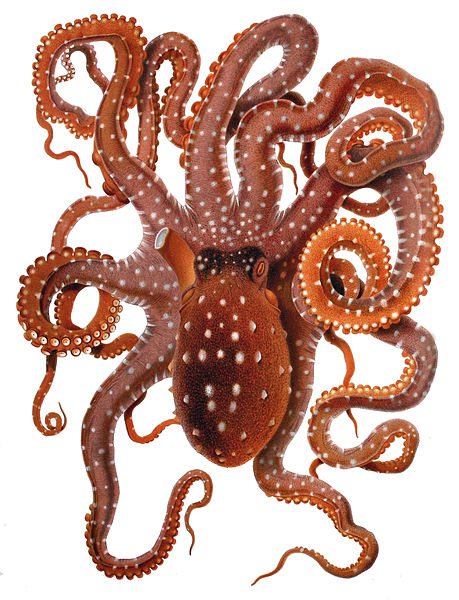
\includegraphics[height=4cm]{Octopus.jpg}
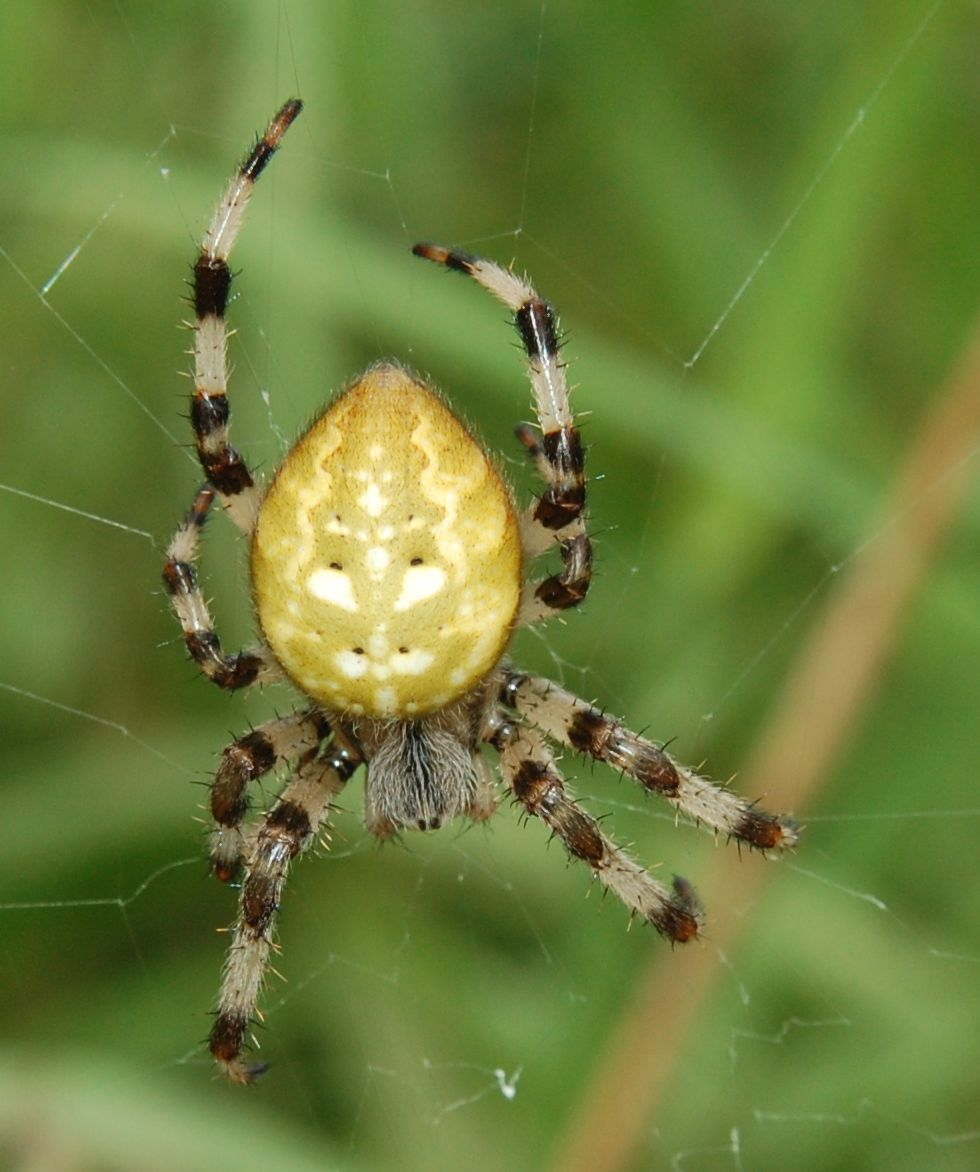
\includegraphics[height=4cm]{Spinne.jpg}


%******************************************************************************************************
\subsection{In uns}
%******************************************************************************************************
nix.

%******************************************************************************************************
\subsection{Additionsverhalten}
%******************************************************************************************************
Keine Besonderheiten.

%******************************************************************************************************
\subsection{Multiplikationsverhalten}
%******************************************************************************************************
Keine Besonderheiten.

%******************************************************************************************************
\subsection{Das kleine Null-plus-Acht}
%******************************************************************************************************
Addition der Zahlen 0 bis 10 mit der 8:
\vspace{\kategoryVspace}

\begin{tabular}{|c|c|c|c|c|c|}
   \hline
   $0 + 8 = 8$ & $1 + 8 = 9$ & $2 + 8 = 10$ & $3 + 8 = 11$ & $4 + 8 = 12$ & $5 + 8 = 13$\\ 
   \hline
               & $6 + 8 = 14$ & $7 + 8 = 15$ & $8 + 8 = 16$ & $9 + 8 = 17$ & $10 + 8 = 18$ \\
   \hline
\end{tabular}

%******************************************************************************************************
\subsection{Das kleine Ein-mal-Acht}
%******************************************************************************************************
Multiplikation der Zahlen 0 bis 10 mit der 8:
\vspace{\kategoryVspace}

\begin{tabular}{|c|c|c|c|c|c|}
   \hline
   $0 * 8 = 0$ & $1 * 8 = 8$ & $2 * 8 = 16$ & $3 * 8 = 24$ & $4 * 8 = 32$ & $5 * 8 = 40$\\ 
   \hline
   & $6 * 8 = 48$ & $7 * 8 = 56$ & $8 * 8 = 64$ & $9 * 8 = 72$ & $10 * 8 = 80$ \\
   \hline
\end{tabular}
%******************************************************************************************************
\subsection{Besonderheiten}
%******************************************************************************************************
Die Acht ist die erste Zahl, die wir nicht nur als Rechteck anordnen können, sondern in mehrere gleichgroße Rechtecke. Die Anordnung als Rechteck:

\begin{tikzpicture}
   \matrix(A) [
      matrix of nodes, 
      nodes in empty cells, 
      nodes={circle, fill=blue, minimum size=5mm},
      column sep=2mm, row sep=2mm
   ] { 
      &&&\\
      &&&\\
   };
\end{tikzpicture}

Dieses Rechteck besteht aus 2 Reihen mit je 4 also $8 = 2 * 4$. Wir können es zerteilen in zwei gleichgroße Rechtecke bestehend jeweils aus 2 Reihen mit je 2 also $8 = (2 * 2)* 2$ wie folgt:

\begin{tikzpicture}
   \matrix(A) [
      matrix of nodes, 
      nodes in empty cells, 
      nodes={circle, fill=blue, minimum size=5mm},
      column sep=2mm, row sep=2mm
   ] { 
      && \node{} ; \fill[white] (0,0) circle(7.5pt); &&\\
      && \node{} ; \fill[white] (0,0) circle(7.5pt); &&\\
   };
\end{tikzpicture}

Wir können das 8-Eck aus einem Quadrat durch abschneiden der Ecken erhalten:

\begin{tikzpicture}
   \node[name=A, draw,minimum size=2cm,regular polygon,regular polygon sides=4, style={
      color = red,
      dotted,
      draw,
      line width = .05cm,
      inner xsep = 2.5cm,
      inner ysep = 0.5cm
   }] (a) {};

   \node[name=A, draw,minimum size=2cm,regular polygon,regular polygon sides=8, style={
      color = green,
      draw,
      line width = .05cm,
      inner xsep = 2.5cm,
      inner ysep = 0.5cm
   }] (a) {};
   
   \node[draw,minimum size=2cm,regular polygon,regular polygon sides=8, style={
      color = black,
      draw=none,
      line width = .01cm,
      inner xsep = 2.47cm,
      inner ysep = 0.5cm
   }] (b) {};
   
   \foreach \x in {1,2,...,8}
   \fill[orange] (b.corner \x) circle[radius=4pt];
   
\end{tikzpicture}

%******************************************************************************************************
\subsection{Zweitteilung geometrisch}
%******************************************************************************************************
Die Zweiteilungen durch Linien am 8-Eck:

\vspace{\kategoryVspace}

\begin{tikzpicture}
   \node[name=A, draw,minimum size=2cm,regular polygon,regular polygon sides=8, style={
      color = green,
      draw,
      line width = .05cm,
      inner xsep = 2.5cm,
      inner ysep = 0.5cm
   }] (a) {};
   
   \node[draw,minimum size=2cm,regular polygon,regular polygon sides=8, style={
      color = black,
      draw=none,
      line width = .01cm,
      inner xsep = 2.47cm,
      inner ysep = 0.5cm
   }] (b) {};
   
   \foreach \x in {1,2,...,8}
      \fill[orange] (b.corner \x) circle[radius=4pt];

   \draw[blue, thick] 
      ({{(-4,0)}} |- a.side 3) -- 
      ({{(10,0)}} |- a.side 3) 
      node[right, above, xshift=-3cm]{$8 = 4+4$};

   \draw[blue, thick] 
      ({{(-4,0)}} |- a.side 4) -- 
      ({{(10,0)}} |- a.side 4) 
      node[right, above, xshift=-3cm]{$8 = 2+6$};


\end{tikzpicture}

So wie

\begin{tikzpicture}
   \node[
      name=A, 
      draw,
      minimum size=2cm,
      regular polygon,
      regular polygon sides=8, 
      shape border rotate=22.5, 
      style={
         color = green,
         draw,
         line width = .05cm,
         inner xsep = 2.5cm,
         inner ysep = 0.5cm
      }
   ] (a) {};
   
   \node[      
      draw,
      minimum size=2cm,
      regular polygon,
      regular polygon sides=8, 
      shape border rotate=22.5, 
      style={
         color = black,
         draw=none,
         line width = .01cm,
         inner xsep = 2.47cm,
         inner ysep = 0.5cm
      }
   ] (b) {};
   
   \foreach \x in {1,2,...,8}
   \fill[orange] (b.corner \x) circle[radius=4pt];
   
   \draw[blue, thick] 
   ({{(-4,0)}} |- a.side 3) -- 
   ({{(10,0)}} |- a.side 3) 
   node[right, above, xshift=-3cm]{$8 = 3+5$};
   
   \draw[blue, thick] 
   ({{(-4,0)}} |- a.side 4) -- 
   ({{(10,0)}} |- a.side 4) 
   node[right, above, xshift=-3cm]{$8 = 1+7$};
   
\end{tikzpicture}

%******************************************************************************************************
%                                                                                                     *
\section{Bildnachweis}
%                                                                                                     *
%******************************************************************************************************
%******************************************************************************************************
\subsection{Stoppschild}
%******************************************************************************************************
Gefunden bei Wikipedia unter \url{https://commons.wikimedia.org/wiki/File:Zeichen_206_-_Halt!_Vorfahrt_gew%C3%A4hren!_StVO_1970.svg}. \textbf{Licensing:} This image is in the public domain according to German copyright law because it is part of a statute, ordinance, official decree or judgment (official work) issued by a German authority or court (§ 5 Abs.1 UrhG).

%******************************************************************************************************
\subsection{Octopus}
%******************************************************************************************************
Gefunden bei Wikipedia unter \url{https://upload.wikimedia.org/wikipedia/commons/thumb/e/eb/Octopus_macropus_Merculiano.jpg/459px-Octopus_macropus_Merculiano.jpg}. \textbf{Licensing:} This work is in the public domain in its country of origin and other countries and areas where the copyright term is the author's life plus 70 years or fewer.


%******************************************************************************************************
\subsection{Spinne}
%******************************************************************************************************
Gefunden bei Wikipedia unter \url{https://de.wikipedia.org/wiki/Vierfleckkreuzspinne#/media/Datei:Araneus_quadratus_070825.jpg}. \textbf{Licensing:} Permission is granted to copy, distribute and/or modify this document under the terms of the GNU Free Documentation License, Version 1.2 or any later version published by the Free Software Foundation; with no Invariant Sections, no Front-Cover Texts, and no Back-Cover Texts. A copy of the license is included in the section entitled GNU Free Documentation License.

%******************************************************************************************************
%                                                                                                     *
\begin{thebibliography}{9}
%                                                                                                     *
%******************************************************************************************************
   \bibitem [MüllerWolfangel2014]{MüllerWolfangel}
      Ute Müller-Wolfangel, Beate Schreiber \emph{Basiswissen Grundschule – Mathematik}
      Bibliographisches Institut 2014, 978-3-411-72063-7 (ISBN)
      
\end{thebibliography}

%******************************************************************************************************
%                                                                                                     *
\begin{large}
    \centerline{\textsc{Symbolverzeichnis}}
\end{large}
%                                                                                                     *
%******************************************************************************************************
\bigskip

\renewcommand*{\arraystretch}{1}

\begin{tabular}{ll}
    $0,1,2,3,4,5,6,7,8,9$          & Ziffern\\
\end{tabular}

\end{document}
